\documentclass[12pt]{article}
\usepackage{lipsum}
\usepackage{authblk}
\usepackage{fancyhdr}

\usepackage{amssymb}
\usepackage{amsmath}

\usepackage[english]{babel}
\usepackage{tikz}
\usetikzlibrary{positioning}
\usepackage[colorlinks=true, urlcolor=blue, linkcolor=black]{hyperref}
\usepackage[doublespacing]{setspace}
\usepackage{geometry}
  \geometry{
    a4paper,
    right=30mm,
    left=30mm,
    bottom=25mm,
    top=25mm
  }

\usepackage{amsmath}
\usepackage{listings}

\pagestyle{fancy}
\setlength{\headheight}{15pt}

\usepackage{algpseudocode}
\usepackage{algorithm}

\usepackage{cite}
\usepackage[nottoc,numbib]{tocbibind}

\usepackage{../presentation/colordef}
\usepackage{../presentation/lvblisting}

\usepackage{wrapfig}

\usepackage{tikz}
\usetikzlibrary{shapes.geometric, arrows}

\tikzstyle{io} = [trapezium, trapezium left angle=70, 
                  trapezium right angle=110, minimum width=3cm, 
                  minimum height=1cm, text centered,
                  draw=black, fill=blue!30]
\tikzstyle{process} = [rectangle, minimum width=3cm,
                       minimum height=1cm, text centered,
                       draw=black, fill=orange!30]
\tikzstyle{decision} = [rectangle, minimum width=3cm,
                        minimum height=1cm, text centered,
                        draw=black, fill=green!30]
\tikzstyle{algo} = [circle, minimum width=1cm, draw=black, fill=orange!30]
\tikzstyle{arrow} = [thick,->,>=stealth]

\renewenvironment{abstract}{%

\begin{center}
\begin{minipage}{0.9\textwidth}
\rule{\textwidth}{1pt}}
{\par\noindent\rule{\textwidth}{1pt}
\end{minipage}
\end{center}}

\begin{document}

\title{Numerical Methods for solving Eigenvalue-Problems}
\author{Thomas Siskos}
\date{}

\begin{titlepage}
  \begin{center}

  \includegraphics[scale=1.25]{../presentation/hulogo.pdf} \par
  {\scshape\LARGE Humboldt Universit{\"a}t zu Berlin \par}

  {\scshape\Large Seminar Paper\par}

  {\huge\bfseries Numerical Methods for solving Eigenvalue-Problems\par}

\vspace{1cm}

  {\Large\itshape Thomas Siskos (580726)\par}

  {\Large\scshape Numerical Introductory Course\par}

  \vfill
  Supervised by: \par
  {\Large Prof. Dr. Brenda L{\'o}pez Cabrera \par}
  \vfill
  {\large \today\par}
  \end{center}

\end{titlepage}

\tableofcontents
\newpage
\listoftables
\listoffigures
\listofalgorithms
\newpage

\section{Motivation}

\begin{singlespacing}
\begin{abstract}
\textbf{Abstract} \\
\small
Eigenvalues and eigenvectors are often the solution to multidimensional optimization problems, however computing them by hand for anything but trivial matrices is most of the time infeasible or inpractical. To this extend we would like to deploy an automated procedure which yields the correct eigenvectors and eigenvalues. We demonstrate the relevance of eigenvalues and eigenvectors by revising two applications from statistics, Principal Component Analysis and Fisher's Linear Discriminant Analysis, which we follow up by investigating four algorithms suited for eigenvalue problems. Finally we provide a compound solution that takes advantage of each algorithms strengths.  
\end{abstract}
\vspace{3mm}
\end{singlespacing}

For many statistical applications eigenvectors provide a formidable solution. Be it dimensionality reduction in terms of a Principal Component Analysis or classification by Fisher's Linear Discriminant Analysis, both come in the guise of optimization problems. But what are eigenvalues and eigenvectors? 

If $A$ is an $n \times n$ matrix, $v$ is a non-zero vector and $\lambda$ is a scalar, such that

\begin{equation}
\label{eigenvalue-def}
Av = \lambda v
\end{equation}

then $v$ is called an \textit{eigenvector} and $\lambda$ is called an \textit{eigenvalue} of the matrix $A$.
An eigenvalue of A is a root of the characteristic equation,

\begin{equation}
\label{eigenvalue-solve}
det\left(A - \lambda I \right) = 0.
\end{equation}

Geometrically speaking, we require a vector which, when multiplied by matrix $A$, will not get rotated but only elongated by a factor $\lambda$.

When confronted with a high-dimensional data matrix $X \in \mathbb{R}^{n \times m}$ an analyst often wishes to find a lower-dimensional representation, while conserving as much of the structure as possible. One way of achieving this goal is to choose a standardized linear combination of features that aim to maximize the variance of the projection $\delta^{\prime} X$. We can formalize this as

\begin{equation}
	\label{pca_obj}
    	max\ \delta^{\prime} Var \left(X\right) \delta \; s.t. \; \sum \delta_i^2 = 1.
\end{equation}

where $X \in \mathbb{R}^{n \times m}; m,n \in \mathbb{N}; \delta \in \mathbb{R}^m$. The Lagrangean that corresponds to the constrained maximization problem in \ref{pca_obj} is

$$
    \mathcal{L}(Var \left(X\right), \delta, \lambda) =
    \delta^{\prime} Var \left(X\right) \delta - \lambda \left(\delta^{\prime}\delta - 1\right),
$$
where $\lambda \in \mathbb{R}^m$

Taking derivatives we obtain the first order condition:
	\begin{align}
	\frac{\partial \mathcal{L}}{\partial \delta} &\stackrel{!}{=} 0 \notag\\
	2Var(X)\delta - 2\lambda_k \delta &\stackrel{!}{=} 0 \notag\\
	Var(X)\delta  &= \lambda_k \delta \notag
	\end{align}

Which is now reduced to a common Eigenvalue problem as posed in (\ref{eigenvalue-def}).


\begin{equation}
\label{pca_sol}
	Y = \Gamma^{\prime} \left(X - \mu\right)
\end{equation}

where $Y \in \mathbb{R}^{n \times m}$ is the matrix of rotations, 
	  $\Gamma \in \mathbb{R}^{m \times m}$ is the matrix of eigenvectors,
	  $\mu \in \mathbb{R}^m$ is the vector of sample means. \cite{MVA}


In section two we lay out the mathematical foundations for the operations we are about to perform. In particular, we will try to reformulate any complicated eigenvalue problem into a straightforward one by diagonalizing the matrix in question, without altering the eigenvalues we would like to compute. We follow these justifications by proposing two main algorithms for computing eigenvalues, first the Jacobi-Method for symmetric matrices, then the QR-Method for arbitrary square matrices in section 3. Additionally, for the QR-Method we define two extensions which try to increase the initial QR-algorithm's speed.
For all algorithms we provide implementations in the \texttt{Python}-programming-language \cite{python, matplotlib, scipy}. In section 4 we will analyse the implemented routines by critically reflecting upon the accuracy of the obtained results as well as their efficiency. In the final section we provide a final algorithm which combines the strengths of the defined procedures by chosing the algorithm that is most fit for the underlying problem.
% ==============================================================================
\section{Similarity Transformations}

In general we want to reformulate the eigenvalue problem of a complicated matrix into an eigenvalue problem of a simple matrix, which yields the same eigenvalues. Simple matrices in our case will be diagonal matrices, since with them it is possible to identify their eigenvalues simply as entries on the main diagonal. Such a transformation that conserves the eigenvalues of a matrix is called a \textit{similarity transformation}. 

Two $n \times n$ matrices $A$ and $B$ are called \textit{similar} if there exists an invertible matrix $P$ such that

\begin{equation}
\label{similarity}
A = P^{-1} B P.
\end{equation}

It is obvious that the similarity relationship is commutative as well as transitive. If $A$ and $B$ are similar, it holds that

\begin{align*}
B - \lambda I &= P^{-1} B P - \lambda P^{-1} I P \notag \\
              &= A - \lambda I.
\end{align*}

 Hence $A$ and $B$ have the same eigenvalues. This fact also follows immediately from the transitivity of the similarity relationship and the fact that a matrix is similar to the diagonal matrix formed from its eigenvalues, as stated in the spectral-decomposition. Important types of similarity transformations are based around orthogonal matrices. If $Q$ is orthogonal and
 
$$ A = Q^{\prime} B Q, $$

$A$ and $B$ are called \textit{orthogonally similar} \cite{NLA}. We will use \textit{orthogonal similarity transformations} to diagonalize matrices we wish to know the eigenvalues of. 

% ==============================================================================
\section{Algorithms}
% ------------------------------------------------------------------------------
\subsection{Jacobi Method}

The \textit{Jacobi-Method} for computing the eigenvalues of a symmetric matrix $A \in \mathbb{R}^{n \times n}$ deploys a sequence of orthogonal similarity transformations that eventually results in
$$ A = P \Lambda P^{-1} \Leftrightarrow \Lambda = P^{-1} A P,$$

where $\Lambda$ is diagonal and $P$ consists of a sequence of matrix multiplications $P = \prod\limits_{k=1}^{K} V_{p_k, q_k}(\theta_k)$ and $V_{p_k, q_k}(\theta_k)$ is of the form proposed in (\ref{givens-rotation}). More specific the \textit{Jacobi iteration} is

\begin{equation}
A^{(k)} = V^{\prime}_{p_k, q_k}(\theta_k) A^{(k-1)} V_{p_k, q_k}(\theta_k),
\end{equation}

where $p_k, q_k$ and $\theta_k$ are chosen such that $A^{k}$ resembles more a diagonal matrix than $A^{k-1}$.  Specifically they will be chosen as to reduce the sum of squares of the off-diagonal elements. As we saw in (\ref{givens-rotation}) it is easy to chose an angle $\theta_k$ in order to introduce a zero in a single Givens rotation. Here we use the rotations in the context of a similarity transformation, so it is a little more complicated.

We require that $a_{pq}^{(k)} = 0$, this implies
\begin{equation}
\label{theta-troubles}
a^{(k-1)}_{pq} (\cos^2\theta - \sin^2\theta) + \left( a^{(k-1)}_{pp} - a^{(k-1)}_{qq} \right) \cos\theta \sin\theta = 0.
\end{equation}
We can use the trigonometric identities
\begin{align*}
\cos(2\theta) &= \cos^2 \theta \sin^2 \theta \\
\sin(2\theta) &= 2 \cos\theta \sin\theta,
\end{align*}

in (\ref{theta-troubles}) we have
$$\tan(2\theta) = \frac{2a^{(k-1)}_{pq}}{a^{(k-1)}_{pp} - a^{(k-1)}_{qq}}.$$

From this we can retrieve the angle and obtain the rotation matrix in each iteration \cite{NLA}.

The algorithm converges if the off-diagonal elements are sufficiently small. The best index pair at a given iteration is the pair $(p, q)$ that satisfies
 
\[
|a^{(k-1)}_{pq}| = \mathop{\max_{i<j}} |a^{(k-1)}_{ij}|.
\]

If this choice is made, the Jacobi Method can be shown to converge \cite{NLA}.

\begin{figure}
\begin{center}
\caption{\href {https://github.com/thsis/NIS18/tree/master/media/plots}{Progress Jacobi-Method}  \protect\includegraphics[scale=0.05]{qletlogo.pdf}}
  \label{j-plot}  
  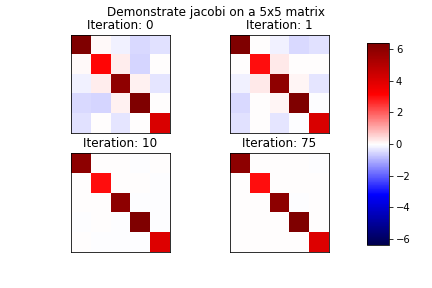
\includegraphics[scale=0.6]{../media/plots/jacobi.png}
\end{center}
\end{figure}


Figure \ref{j-plot} visualizes the progress of the \textit{Jacobi}-method on a symmetric $5 \times 5$ matrix. As we can see, in the first iteration the element $a_43$ is eliminated. In the subsequent operations the \textit{Jacobi}-method continues to eliminate any non-zero entries on the off-diagonal until the algorithm convergences after 10 iterations.

\begin{algorithm}
\caption{\texttt{jacobi}}
\label{j-algo}
\begin{algorithmic}[1]
  \Require symmetric matrix $A$
  \Ensure $0 < precision < 1$
  \Statex \textbf{initialize: } $L \gets A$; $U \gets I$; $L_{max} \gets 1$
  \While{$L_{max} > precision$}
    \State Find indices $i$, $j$ of largest value in lower triangle of $abs(L)$
        \State $L_{max} \gets L_{i,j}$
            \State $\alpha \gets \frac{1}{2}\cdot \arctan(\frac{2A_{i, j}}{A_{i, i}-A_{j, j}})$
    \State $V \gets I$
    \State $V_{i, i}, V_{j, j} \gets \cos \alpha$; $V_{i, j}, V_{j, i} \gets -\sin \alpha, \sin \alpha$
    \State $A \gets V^{\prime} A V$; $U \gets UV$

  \EndWhile\\
  \Return $diag(A),\; U$
\end{algorithmic}
\end{algorithm}

% ------------------------------------------------------------------------------
\subsection{QR-Method}

The most widely used algorithm to extract eigenvalues is the so called \textit{QR}-method. The most important advantage of the \textit{QR}-method over the \textit{Jacobi}-method is that it can be applied to non-symmetric matrices. Note however, that it is simpler for symmetric matrices, since the eigenvalues are real-valued.

The \textit{QR}-method to extract the eigenvalues of a square matrix $A \in \mathbb{R}^{n \times n}$ is performed by first computing the titular \textit{QR} decomposition of $A$.

\begin{equation}
\label{qr_a}
A = QR,
\end{equation}

where $Q$ is an orthogonal and $R$ is an upper triangular matrix. Then define the \textit{QR} iteration as

\begin{equation}
\label{qr-method}
  A^k = Q_{k-1}^{\prime} A_{k-1} Q_{k-1} = R_{k-1}Q_{k-1}
\end{equation}

Note hereby that all matrices in the sequence $\{A_k\}$ share the same eigenvalues, since this procedure is a similarity transformation due to $Q$'s orthogonality. Additionally, in an implementation it is usually preferable to compute the \textit{QR}-iteration in the way shown at the rightmost part of equation (\ref{qr-method}) \cite{NME}. Although, mathematically, each statement is exactly identical there is a practical difference in due to computational imperfections and limited machine precision. The reason being that the computation of $Q_{k-1}^{\prime} A_{k-1} Q_{k-1}$ obviously requires two matrix multiplications whereas the result of $R_{k-1}Q_{k-1}$ can be readily obtained by one. When combining multiple steps over a long sequence of \textit{QR} iterations the additional computations lead to additional rounding errors, which can have an influence on the accuracy of the obtained results. Additionally, less computations lead of course to a faster procedure in general. 

\begin{figure}
\begin{center}
\label{qrm1-plot}
\caption{\href {https://github.com/thsis/NIS18/tree/master/media/plots}{Progress basic QR-Method}  \protect\includegraphics[scale=0.05]{qletlogo.pdf}}
  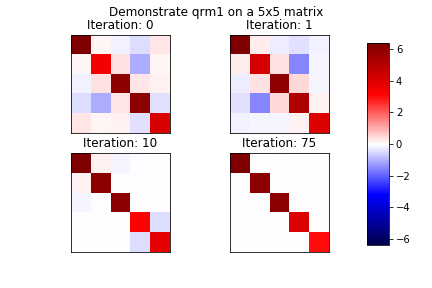
\includegraphics[scale=0.6]{../media/plots/qrm1.png}
\end{center}
\end{figure}

Figure \ref{qrm1-plot} visualizes the progress of the basic \textit{QR}-method on the same $5 \times 5$ matrix as in Figure \ref{j-plot}. Compared to the \textit{Jacobi}-method it does not explicitly pick a single element that will be eliminated per iteration. Instead, the \textit{QR}-method extracts the eigenvalues by a process that is called "chasing". By that we mean that alternating steps are being performed, which create non-zero eintries in positions $(i+2, i)$, $(i+3, i)$ and $(i+3, i+1)$ and restore them to zero, as the nonzero entries are moved farther down the matrix \cite{NLA}. We can also see that compared to the \textit{Jacobi}-Method, so far, the \textit{QR}-algorithm lacks in speed. Where the \textit{Jacobi}-method was almost done diagonalizing the matrix in iteration 10, the basic \textit{QR}-algorithm still had multiple non-zero entries left. Thus we would like to make minor improvements on the algorithm's efficiency.
\begin{algorithm}
\caption{\texttt{QRM1}}
\label{qr1-meth}
  \begin{algorithmic}[1]
    \Require square matrix $A$
    \Statex \textbf{initialize: } $conv \gets False$
    \While{not $conv$}
      \State $Q, R \gets$ QR-Factorization of $A$
      \State $A \gets RQ$
      \If{$A$ is diagonal}
        \State $conv \gets \texttt{True}$
      \EndIf
    \EndWhile\\
    \Return $diag\left(A\right),\; Q$
  \end{algorithmic}
\end{algorithm}


\subsubsection{Hessenberg Variant}

In order to speed up the \textit{QR}-method it is advisable to transform the matrix to its upper \textit{Hessenberg} form. A matrix $A$ is of upper \textit{Hessenberg} form if it is upper triangular except for the first subdiagonal, which may be non-zero. In particular $a_{ij} = 0\; \forall i > j + 1$:
$$
\begin{bmatrix}
X & X & X  & \dots &  X & X\\
X & X & X &  \dots &  X & X\\
0 & X & X &  \dots &  X & X\\
0 & 0 & X &  \dots &  X & X \\
\vdots &  \vdots & & \ddots  & \vdots  & \vdots\\
0 & 0 & 0 &  \dots &  X & X \\
\end{bmatrix}$$

A matrix can be reduced to \textit{Hessenberg} form in a finite number of similarity transformations using Householder transformations or Givens rotations. For symmetric matrices the transformation into a \textit{Hessenberg}-form results in a tridiagonal matrix. But even for non-symmetric matrices, the \textit{Hessenberg}-form allows a large saving in subsequent computations. After the transformation we can deploy the previously defined \textit{QR}-method \cite{NLA}.  

\begin{figure}[H]
\begin{center}
\caption{\href {https://github.com/thsis/NIS18/tree/master/media/plots}{Progress Hessenberg-QR-Method}  \protect\includegraphics[scale=0.05]{qletlogo.pdf}}
  \label{qr2-plot}  
  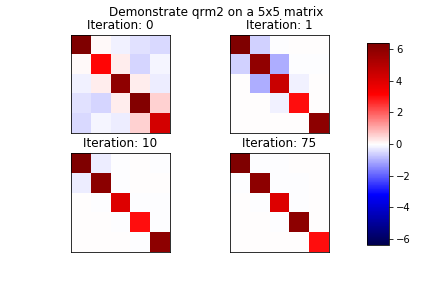
\includegraphics[scale=0.6]{../media/plots/qrm2.png}
\end{center}
\end{figure}

Figure \ref{qr2-plot} visualizes the progress of the \textit{Hessenberg} variant of the \textit{QR}-method. In order to make it comparable to the previous algorithms the same $5 \times 5$-dimensional matrix is being evaluated. We can readily see, that the transformation to \textit{Hessenberg}-form results in a tridiagonal matrix. This facilitates computations and explains the vastly improved resulting matrix after 10 iterations compared to the basic \textit{QR}-method. However, it still does not match the progress of the \textit{Jacobi}-method after the same number of iterations.


\begin{algorithm}
\caption{\texttt{QRM2}}
\label{qr2-meth}
\begin{algorithmic}[1]
  \Require square matrix $A$
  \State $A \gets \texttt{hessenberg(}A\texttt{)}$
  \State continue with: \Call {QRM1} A
\end{algorithmic}
\end{algorithm}


\subsubsection{Accelerated Variant}

We could already improve the \textit{QR}-method and cut down on computational cost. However, we still cannot match the results of the \textit{Jacobi} method. To this effect we present the final adjustment on the \textit{QR}-method to improve convergence speed. The general idea is, that we deliberately create an additional zero entry on the main diagonal by subtracting a scalar on each element, perform the \textit{QR}-iteration and finally undo the subtraction. In particular, we define

\begin{equation}
\label{qrm3-prop}
T^{m} = \begin{bmatrix}

\alpha^{m}_1 & \beta^{m}_1  & 0            & 0            & \dots            & 0                                  \\
\beta^{m}_1  & \alpha^{m}_2 & \beta^{m}_2                                                                         \\
0            & \beta^{m}_2  & \alpha^{m}_3 & \beta^{m}_3  &                  & \vdots                             \\
             &              & \ddots       & \ddots       & \ddots                                                \\
             &              &              &              & \beta^{m}_{n-2}  & \alpha^{m}_{n-1} & \beta^{m}_{n-1} \\
0            &              &              &              &                  & \beta^{m}_{n-1}  & \alpha^{m}_n    \\

\end{bmatrix}
\end{equation}


\begin{align*}
T^{m}       &= T - t _{n, n} I \\
T^{m}       &= QR \\
T^{m+1}     &= T^{m} + t _{n, n} I
\end{align*}

After this we can define the accelerated iteration step as
\begin{align}
\label{qrm3}
R_m &= Q^{\prime}_m\left(T_m - \alpha_n^{m}I\right) \\
T_{m+1} &= Q^{\prime}_m\left(T_m - \alpha_n^{m}I\right)Q_m + \alpha_n^{m}I \\
        &= Q^{\prime}_m T_m Q_m
\end{align}

Again $T_{m+1}$ is similar to $T_m$. 

\begin{figure}[H]
\begin{center}
\caption{\href {https://github.com/thsis/NIS18/tree/master/media/plots}{Progress Accelerated QR-Method}  \protect\includegraphics[scale=0.05]{qletlogo.pdf}}
  \label{qr3-plot}
  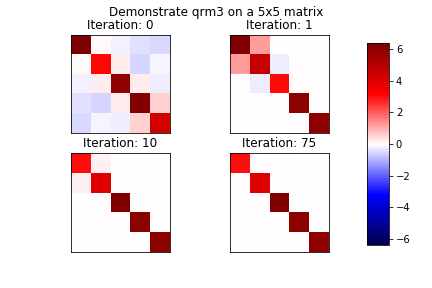
\includegraphics[scale=0.6]{../media/plots/qrm3.png}
\end{center}
\end{figure}

Figure \ref{qr3-plot} visualizes the progress of the accelerated \textit{QR}-method. For comparability, the matrix used is the same $5 \times 5$ matrix as before. Most notably is, that the accelerated method still performs worse than the \textit{Jacobi} method. So far results seem similar compared to the \textit{Hessenberg} variant of the \textit{QR}-method. The case can be made that the accelerated method performs considerably better than the basic \textit{QR}-method and slightly better than the \textit{Hessenberg} variant after 10 iterations than the. Howbeit, this claim warrants further analysis. 

\begin{algorithm}
\begin{algorithmic}[1]
\caption{\texttt{QRM3}}
\Require square matrix $A \in \mathbb{R}^{p \times p}$
\State $T \gets \texttt{hessenberg}(A),\ conv \gets False$
\While{not $conv$}
    \State $Q, R \gets$ QR-Factorization of $T - t_{p-1, p-1} I$
    \State $T \gets RQ + t_{p-1, p-1}I$
    \If{$T$ is diagonal}
        \State $conv \gets True$
    \EndIf
\EndWhile\\
\Return $diag\left(T\right),\; Q$
\end{algorithmic}
\end{algorithm}

% ==============================================================================
\section{Analysis}

%%%%%%%%%%%%%%%%%%%%%%%%%%%%%%%%%%%%%%%%%%%%%%%%%
%%%%%%%%%%%%%%%% CONTINUE ME %%%%%%%%%%%%%%%%%%%%%%
%%%%%%%%%%%%%%%%%%%%%%%%%%%%%%%%%%%%%%%%%%%%%%%%%%%%%

% ------------------------------------------------------------------------------
\subsection{Accuracy}
\begin{table}
\caption{Unit tests accross matrix-sizes}
\begin{tabular}{cc}
awesome & sauce \\
\hline
nothing & to \\
see & here

\end{tabular}
\end{table}
% ------------------------------------------------------------------------------
\subsection{Efficiency}

\begin{figure}
\begin{center}
\caption{\href {https://github.com/thsis/NIS18/blob/master/tests/tests_eigen.py}{Unit-tests: Iterations}  \protect\includegraphics[scale=0.05]{qletlogo.pdf}}
  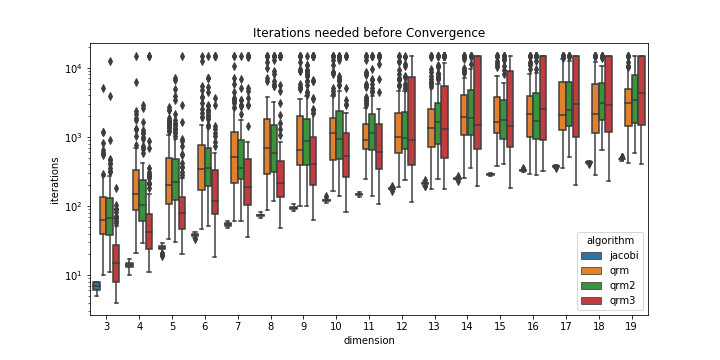
\includegraphics[width=\textwidth, height=5cm]{../media/plots/iterations_boxplot.png}
\end{center}
\end{figure}


% ==============================================================================
\section{Conclusion}
\begin{figure}
\centering
\caption{Decision process of final eigenvalue routine}
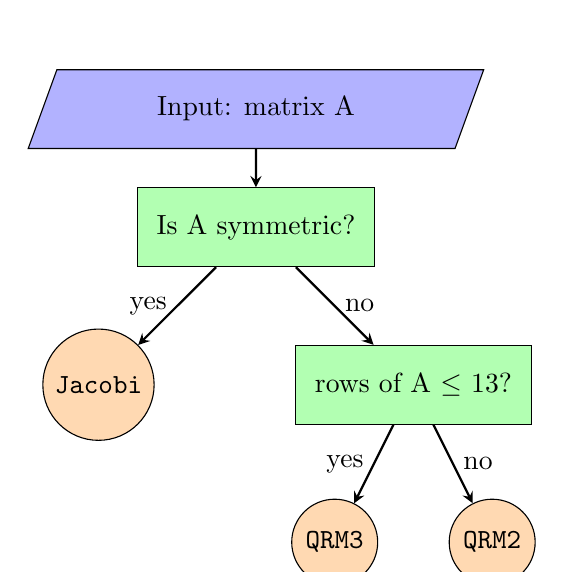
\begin{tikzpicture}
\node (in1) [io] {Input: matrix A};
\node (dec_sym) [decision, below of=in1, yshift=-0.5cm] {Is A symmetric?};
\node (algo1) [algo, below of=dec_sym, xshift=-2cm, yshift=-1cm] {\texttt{Jacobi}};
\node (dec_small) [decision, below of=dec_sym, xshift=2cm, yshift=-1cm] {rows of A $\leq$ 13?};
\node (algo2) [algo, below of=dec_small, xshift=-1cm, yshift=-1cm] {\texttt{QRM3}};
\node (algo3) [algo, below of=dec_small, xshift=1cm, yshift=-1cm] {\texttt{QRM2}};

\draw [arrow] (in1) -- (dec_sym);
\draw [arrow] (dec_sym) -- node[anchor=east] {yes} (algo1);
\draw [arrow] (dec_sym) -- node[anchor=west] {no} (dec_small);
\draw [arrow] (dec_small) -- node[anchor=east] {yes} (algo2);
\draw [arrow] (dec_small) -- node[anchor=west] {no} (algo3);
\end{tikzpicture}
\end{figure}
% ==============================================================================
\newpage
\section{Appendix}
\subsection{Householder-Reflections}

Our goal is still to diagonalize a matrix in order to programmatically extract it's eigenvalues. So far we have seen that there exist such transformations that conserve the eigenvalues of a given matrix. However, we require transformations that, additionally, eliminate non-zero entries on the off-diagonal elements of said matrix. A greedy technique, that eliminates all but the first elements of a vector is proposed in the form of Householder-Reflections.

Let $u$ and $v$ be orthonormal vectors and let $x$ be a vector in the space spanned by $u$ and $v$, such that
$$x = c_1 u + c_2 + v$$ 
for some scalars $c_1$ and $c_2$. The vector 
$$\tilde{x}=-c_1 u + c_2 v$$ 
is a \textit{reflection} of x through the line difined by the vector u. Now consider the matrix

\begin{equation}
P = I - 2 uu^{\prime}.
\end{equation}
Note that
\begin{align*}
Px &= c_1 u + c_2 v - 2c_1 uuu^{\prime} - 2 c_2 v uu^{\prime} \\
   &= c_1 u + c_2 v - 2c_1 u^{\prime}uu - 2 c_2 u^{\prime} v u \\
   &= -c_1 u + c_2 v\\
   &= \hat{x}.
\end{align*}

The matrix $P$ is called a reflector. The usefulness of Householder-Reflections stems from the fact that it is easy to transform a vector of the form

$$x = (x_1, x_2, \dots, x_n)$$

into a vector
$$\hat{x} = (\hat{x}_1, 0, \dots, 0).$$

If $Qx = \hat{x}$, then $||x||_2 = ||\hat{x}||_2$ and thus $\hat{x_1} = \pm ||x||_2$, since it is the only non-zero entry. To construct the reflector let
\begin{equation}
\label{house-con}
v = (x_1 + sign(x_1)||x||_2, x2, \dots, x_n)
\end{equation}
and $u = \frac{v}{||v||_2}$ \cite{NLA}. We use the $sign$-function, which simply returns the sign of its argument in order to avoid the numerical problem known as \textit{catastrophic cancellation}. It can occur when adding two very close, but different, floating point numbers of differing signs. In some unfortunate cases both of these numbers get represented by the same computer number and, because of their opposing signs cancel each other out. In our case this would mean, that we reflect the vector onto the origin. Fortunately, by making use of the \textit{sign} function we can make sure that both summands will share the same sign, thus mitigating any concerns about catastrophic cancellation.

We use reflectors to compute the so called $QR$ factorization of an aribitrary square matrix $A \in \mathbb{R}^{n \times n}$.

\begin{equation}
\label{QR-prop}
A = QR
\end{equation}

where $Q$ is orthogonal and $R$ is upper triangular. We use Householder transformations to reflect the $i^{th}$ column and produce zeros below the $(i, i)$ element. The QR-factorization of a matrix $A \in \mathbb{R}^5$ would therefore consist of five Householder-reflections with $Q=P_5 P_4 P_3 P_2 P_1$. The number of computations for the \textit{QR} factorization in this fashion is $2n^3 / 3$ multiplications and $2n^3 / 3$ additions \cite{NLA}.  
% ------------------------------------------------------------------------------
\subsection{Givens-Rotations}

\begin{wrapfigure}[7]{r}{0.3\textwidth}
\centering
\caption{Rotation of \textit{x}}
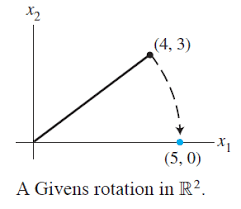
\includegraphics[scale=0.5]{../media/plots/givens.png}
\end{wrapfigure}

Another way of forming the \textit{QR}-factorization is by using orthogonal transformations which rotate a vector in a way such that a specific element becomes 0 and only one other element in the vector being changed. These transformations are called \textit{Givens transformations, Givens Rotations} or \textit{Jacobi transformations}

Using orthogonal transformations we can also rotate a vector in such a way that a specified element becomes 0 and only one other element in the vector is changed. The basic idea can be seen in a two-dimensional space. We wish to rotate the vector $x = (x_1, x_2)$ to $\tilde{x} = (\tilde{x_1}, 0)$ as with a reflector.

It is easy to see that the orthogonal matrix 
$$Q=\begin{bmatrix}
\cos\theta & \sin\theta \\
-\sin\theta & \cos\theta
\end{bmatrix}$$

performs the desired rotation, if $\cos\theta = \frac{x_1}{||x||_2}$ and $\sin\theta = \frac{x_2}{||x||_2}$

In general, we can construct an orthogonal $matrix V_{pq}$, that will transform the vector $$x = (x_1,\dots, x_p, \dots x_q, \dots, x_n)$$ to $$\tilde{x} = (x_1,\dots, \tilde{x}_p, \dots 0, \dots, x_n)$$. The matrix that does this is
\begin{equation}
\label{givens-rotation}
V_{pq}(\theta) = \begin{bmatrix}
                      1 \\
                        & \ddots \\
                        &        & \cos\theta    &        & \sin\theta  \\
                        &        &               & \ddots     \\
                        &        & -\sin\theta   &        & \cos\theta   \\
                        &        &               &        &            &  \ddots \\
                        &        &               &        &            &         & 1 \\                      
                 \end{bmatrix}
\end{equation}
	where $\cos\theta = \frac{x_p}{||x||}$ and $\sin\theta = \frac{x_q}{||x||}.$
	
A rotation matrix is therefore the same as an identitiy matrix, in which we change four elements \cite{NME}. We will use Givens rotations primarily in the Jacobi-Method.


\subsection{Eigenvalue Routines}
  \lstinputlisting[language=Python]{../algorithms/helpers.py}
  \lstinputlisting[language=Python]{../algorithms/eigen.py}
  \newpage
\subsection{Analysis: Figures}
  \lstinputlisting[language=Python]{../analysis/analysis.py}
  \newpage    
\subsection{Analysis: Unit tests}
  \lstinputlisting[language=Python]{../tests/tests_eigen.py}
  \newpage
% ==============================================================================
\bibliographystyle{apalike}
\bibliography{references}

\end{document}